\newpage
\section{Privacy Protection against Real-World Apps}
\label{sec:protecting_up}


In Figure~\ref{fig:intro_case_study_uber}, we showed how \framework{} can be effectively used to protect user privacy while they are using Uber. In this section, we use three more real-world Android apps to showcase privacy advantages of \framework{}.

\subsection{com.katana.facebook (v404.0.0.35.70)}
\label{sec:fb_case_study}
 
During the experiment, while scrolling through posts in the Facebook app's \textit{Home} activity and without engaging any other app features, \framework{}'s \textit{Resource Access Log Reporter} recorded instances of the Facebook app accessing audio permission as shown in Figure~\ref{fig:case-study-facebook}(a). On further investigation, we found that the Facebook app was using \texttt{MediaRecorder} to access the device microphone. Moreover, the Android's privacy indicator~\cite{andPrivacyIndicator} (green dot), which indicates active use of the device microphone, did not appear when \framework{} logged the use of audio permission. We found this surprising.

We were able to repeat this behavior with a custom mobile app i.e. we used \texttt{MediaRecorder} API to successfully record audio while Android's privacy indicator did not show up. We believe it is a bug in Android's privacy indicator implementation. We have reported this to Android and plan to open source this custom app responsibly.

Hence, \framework{} was able to detect microphone usage that was not indicated by Android. Moreover, \framework{} successfully spoofed audio data requested by the Facebook app. 

Similar to the unexpected microphone access, \framework{} also logged instances of calendar data access by the Facebook app while searching for nearby events. The app reads user's calendar events to display their availability when the user is viewing nearby events. Users can configure \framework{} to manipulate calendar data in a way that allows the Facebook app to receive information about their availability without compromising sensitive details about individual events. This involves spoofing fields like event name and location. \framework{} could spoof the app's request for calendar data by providing a list of manipulated events.

\begin{figure}[t]
    \centering
    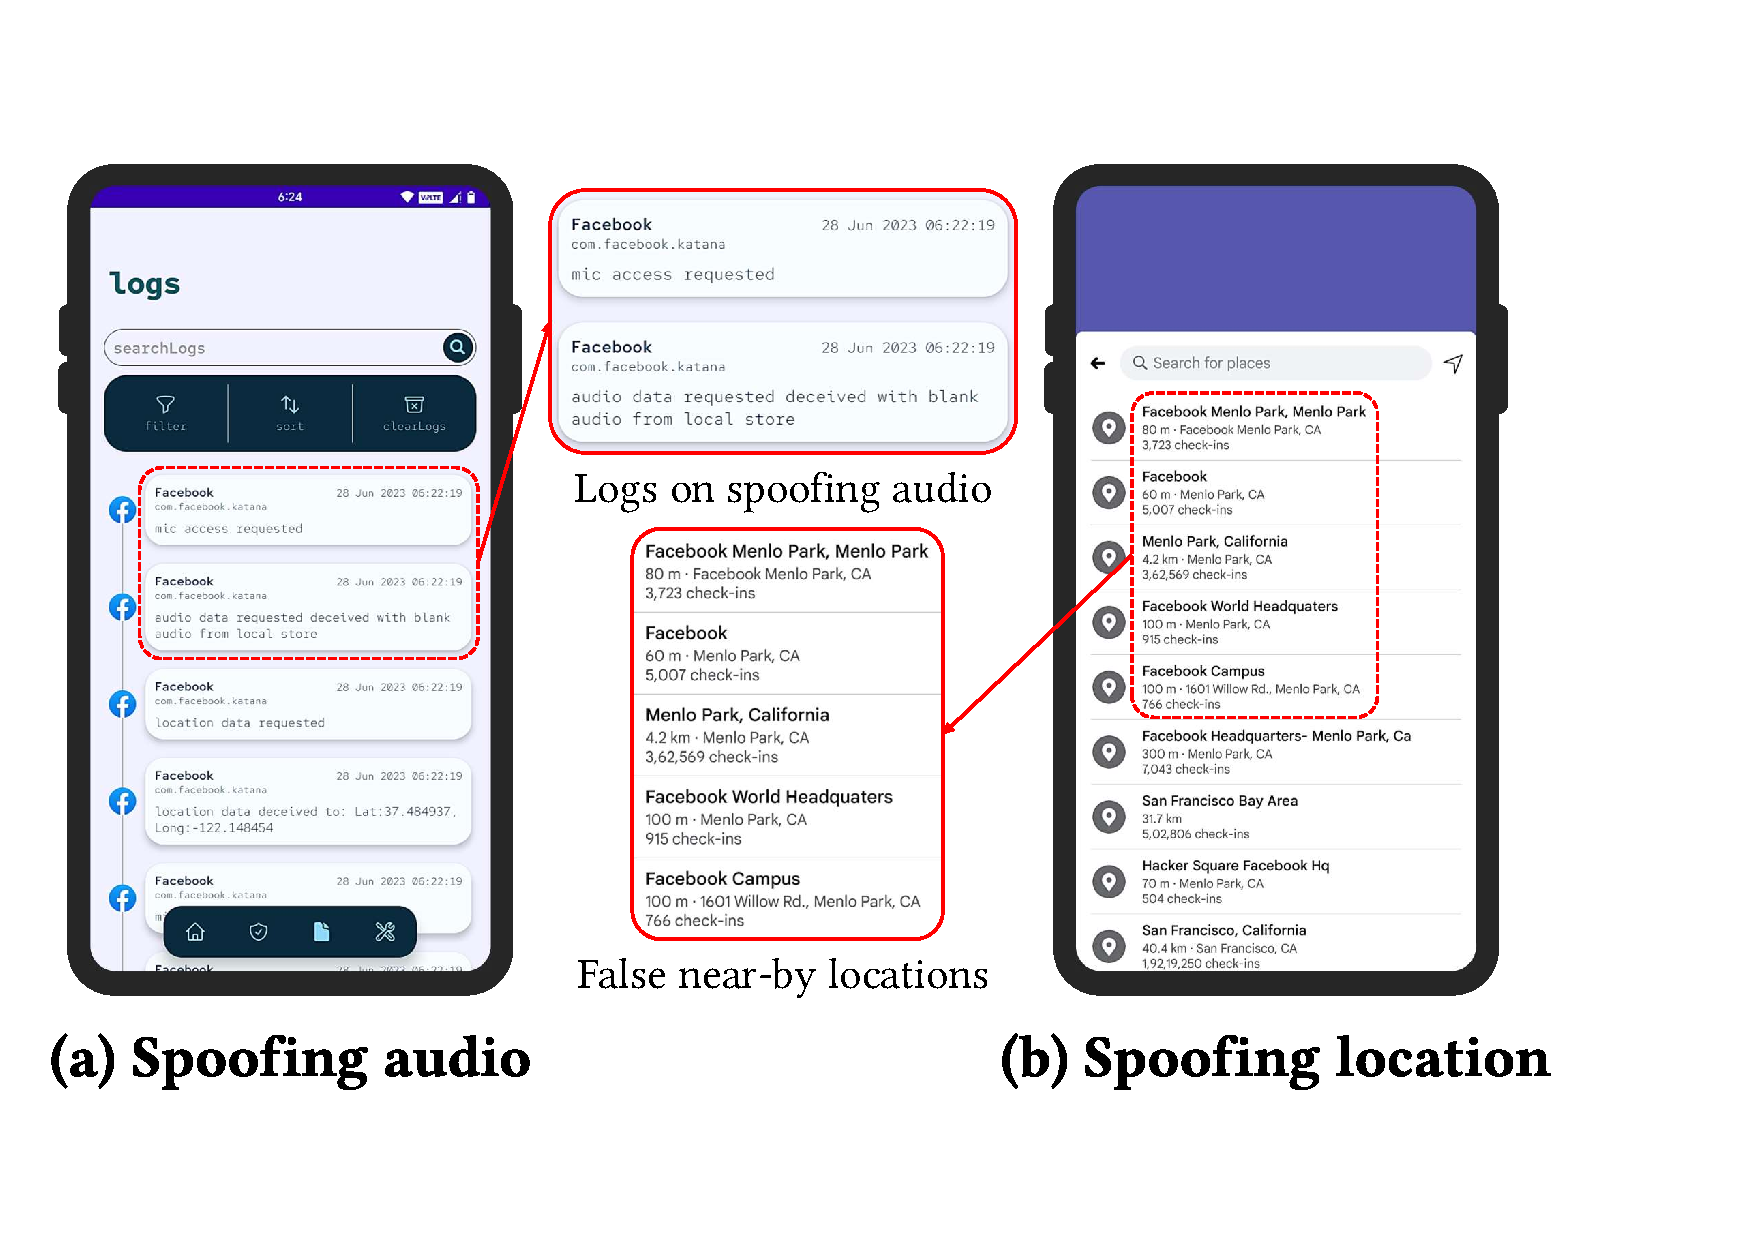
\includegraphics[width=0.75\linewidth]{Figures/Case Studies/facebook_screenshots.pdf}
    \caption{Screenshots demonstrating deceiving location and audio data using \framework{} for the Facebook app.}
    \label{fig:case-study-facebook}
\end{figure}

Nearby events were listed using user's location data. As shown in Figure~\ref{fig:case-study-facebook}(b), we could effectively spoof the fine-grained GPS location data with a nearby location ensuring that the reported nearby places and events were same without compromising user's exact location. 

\subsection{com.snapchat.android (v12.24.0.34)}
\label{sec:sc_case_study}

\begin{figure}[t]
    \centering
    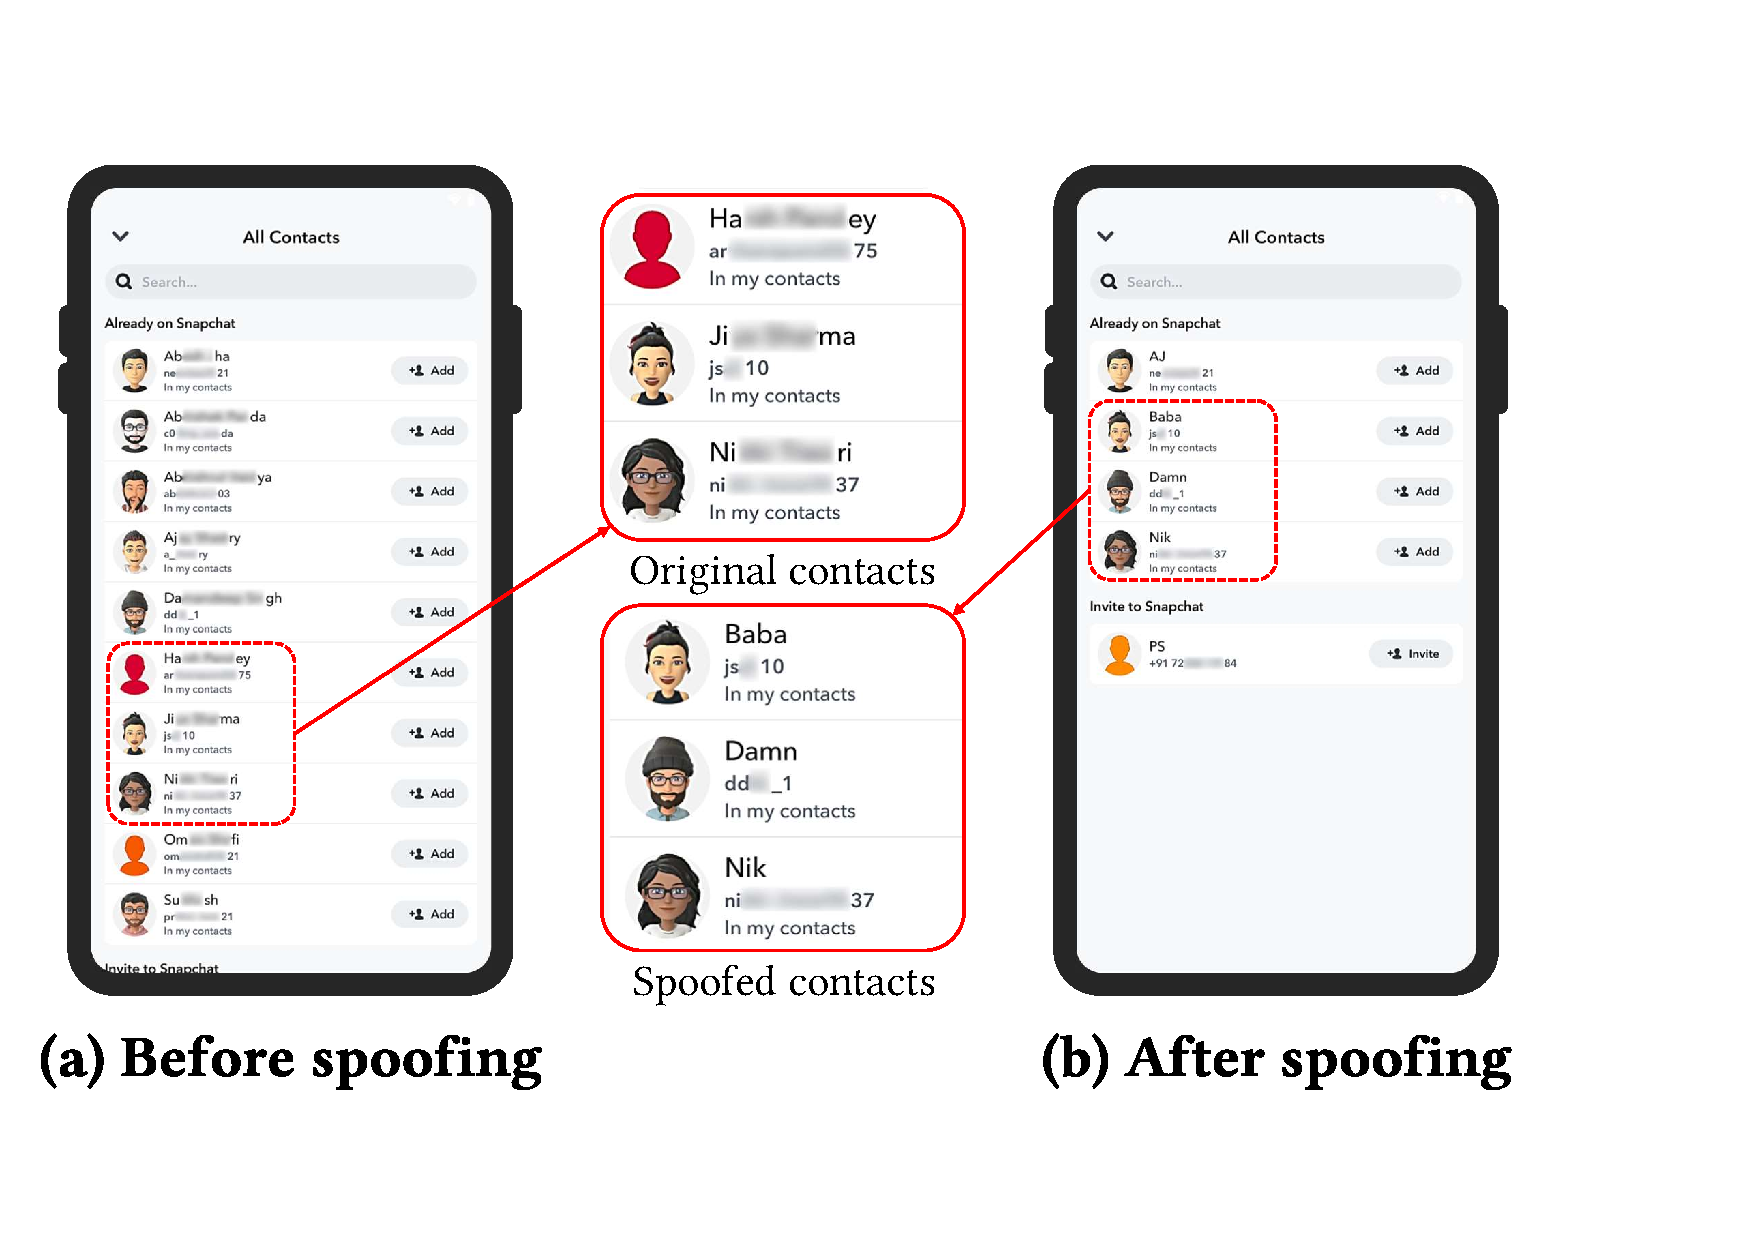
\includegraphics[width=0.75\linewidth]{Figures/Case Studies/snapchat_screenshots.pdf}
    \caption{Screenshots demonstrating how user can share spoofed contacts using WhiteLie with Snapchat.}
    \label{fig:case-study-snapchat}
\end{figure}

Snapchat has a feature called \textit{Snap Map}, which utilizes the device's GPS and other sensors to display user avatars on a map, showcasing real-time physical activities. While Snapchat does provide \textit{Ghost Mode} as an option to refrain from sharing location and sensor data, it sacrifices \textit{SnapMap} features that rely on this information. Furthermore, \textit{Ghost Mode} does not guarantee that the app is not accessing the data. 

\framework{} successfully spoofed device's GPS location and \texttt{READ\_CONTACTS} by utilizing a list of contacts specified in \framework{}'s \textit{Deceit} section as shown in Figure \ref{fig:case-study-snapchat}(b). Users can thus limit the information they want to share with Snapchat and still use Snap Map feature.

\subsection{com.truecaller (v12.54.7)}
\label{sec:tc_case_study}
Truecaller provides sender information about incoming text messages to highlight known spammers. With Truecaller, users can ignore spam messages. But to use this feature, users have to give permission to the app to read all their messages. We used \framework{} to successfully spoof message content while retaining the phone number from which the message was received. This way users can retain control over the privacy of their messages while still identifying whether senders are known spammers as shown in
Figure~\ref{fig:case-study-truecaller}(b).

\begin{figure}[t]\centering
    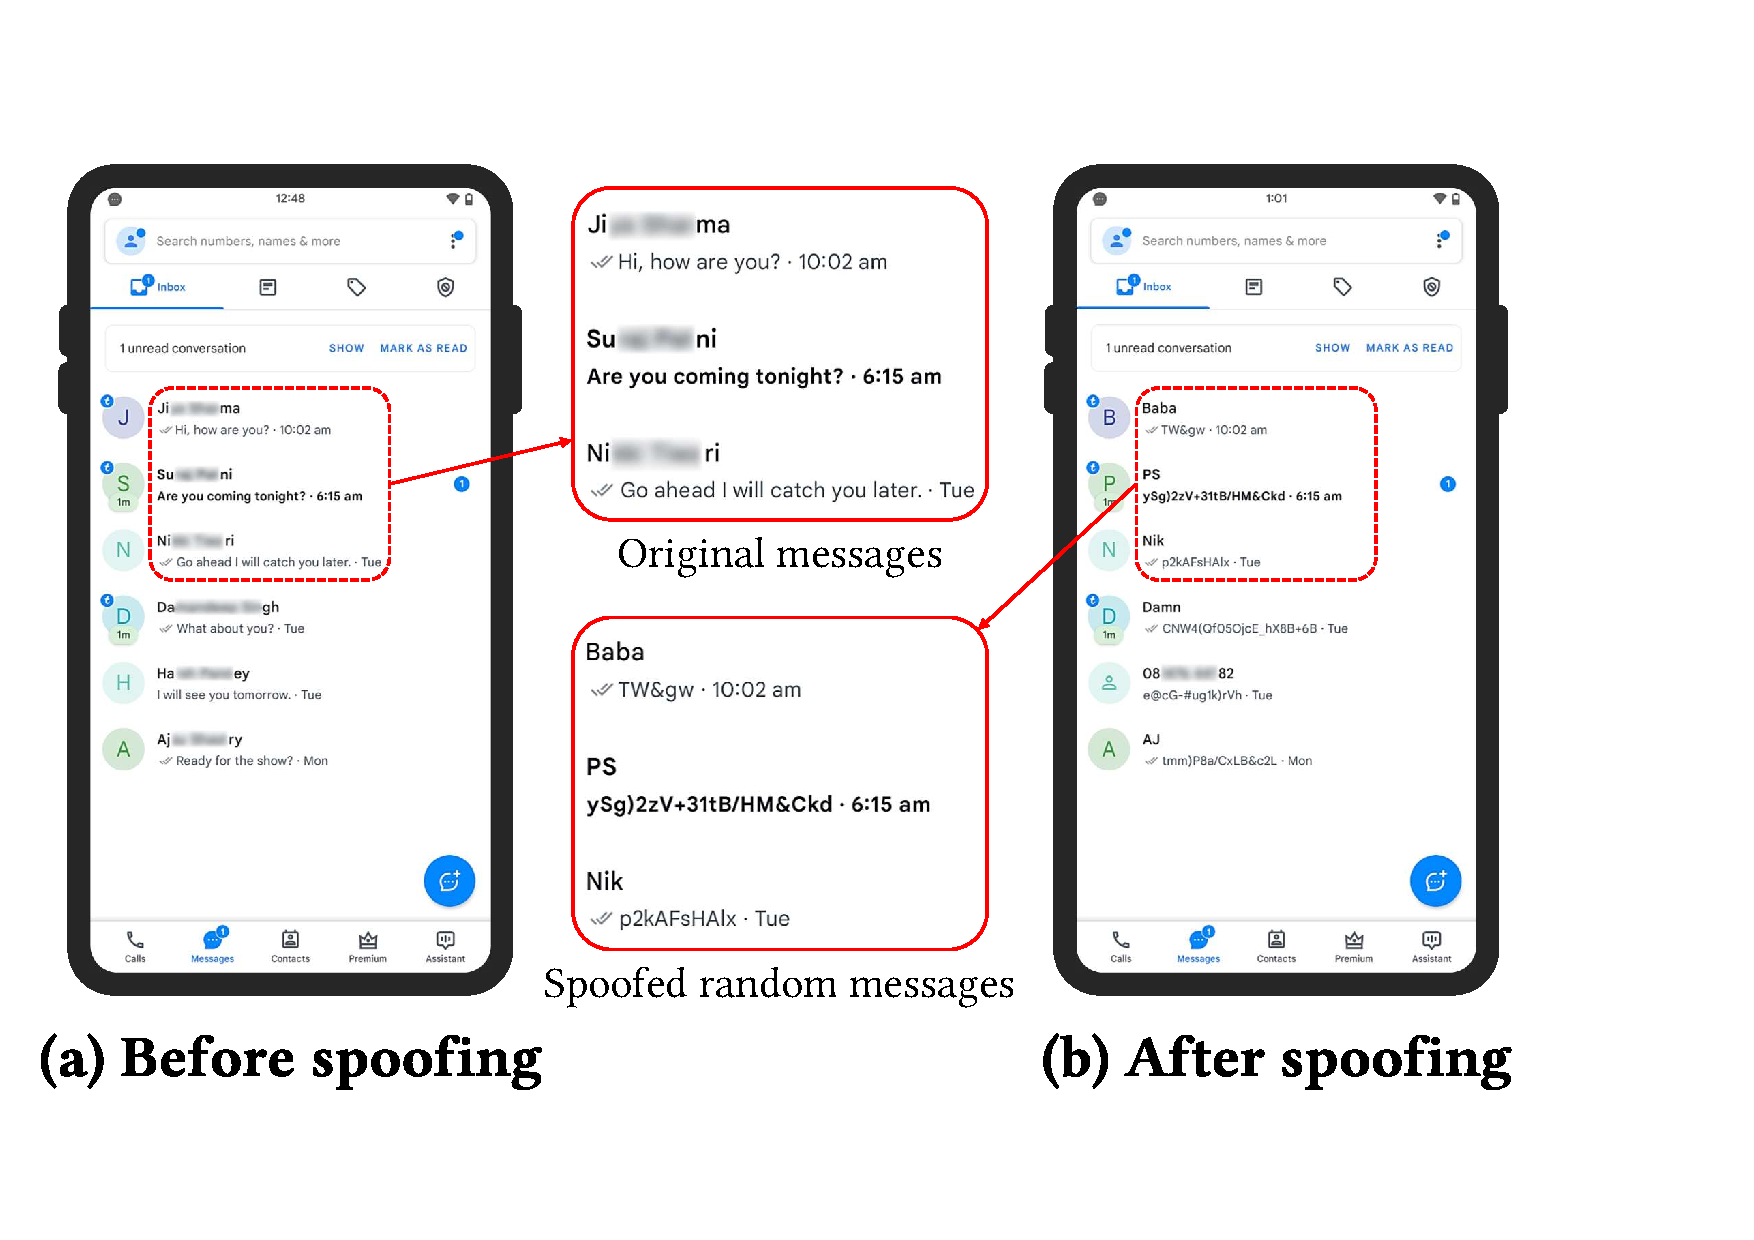
\includegraphics[width=0.75\linewidth]{Figures/Case Studies/truecaller_screenshots.pdf}
    \caption{Screenshots demonstrating how a user can share spoofed SMS using WhiteLie with Truecaller app.}
    \label{fig:case-study-truecaller}
\end{figure}

\textit{Overall, this section shows that \framework{} empowers users to fully use the app features while controlling the information that they share with the apps.}
